\chapter{Implementation}
\label{cha:implementation}

Implementation:
\begin{itemize}
    \item Backend architecture
    \item Android
    \item iOS
\end{itemize}


\vspace{0.5cm}

\section{Backend}

\subsection{Architecture}

In this section we will focus on the architecture and our decision for the backend and its communication.
We build a RESTful API which allows the clients to communicate with the backend in a JSON\footnote{\url{http://json.org/index.html}} format. 

\begin{center}
    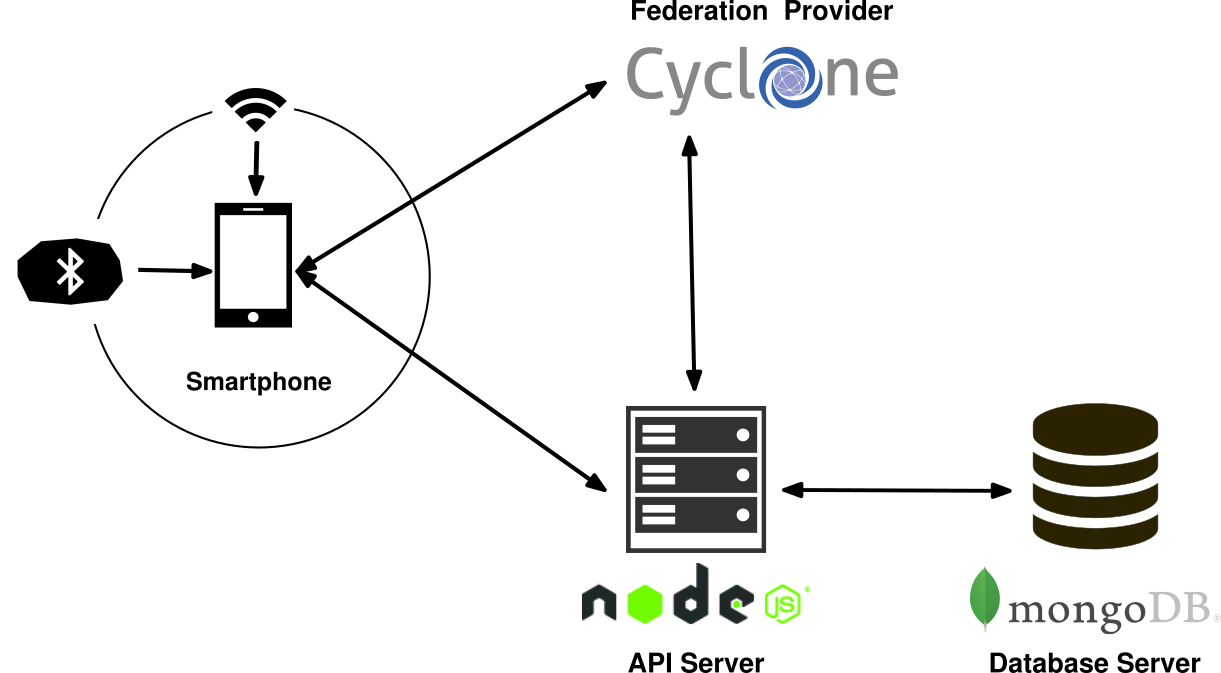
\includegraphics[width=\textwidth]{architecture_v02}\\
\end{center}

\subsection{CYCLONE Federation Provider}

\begin{center}
    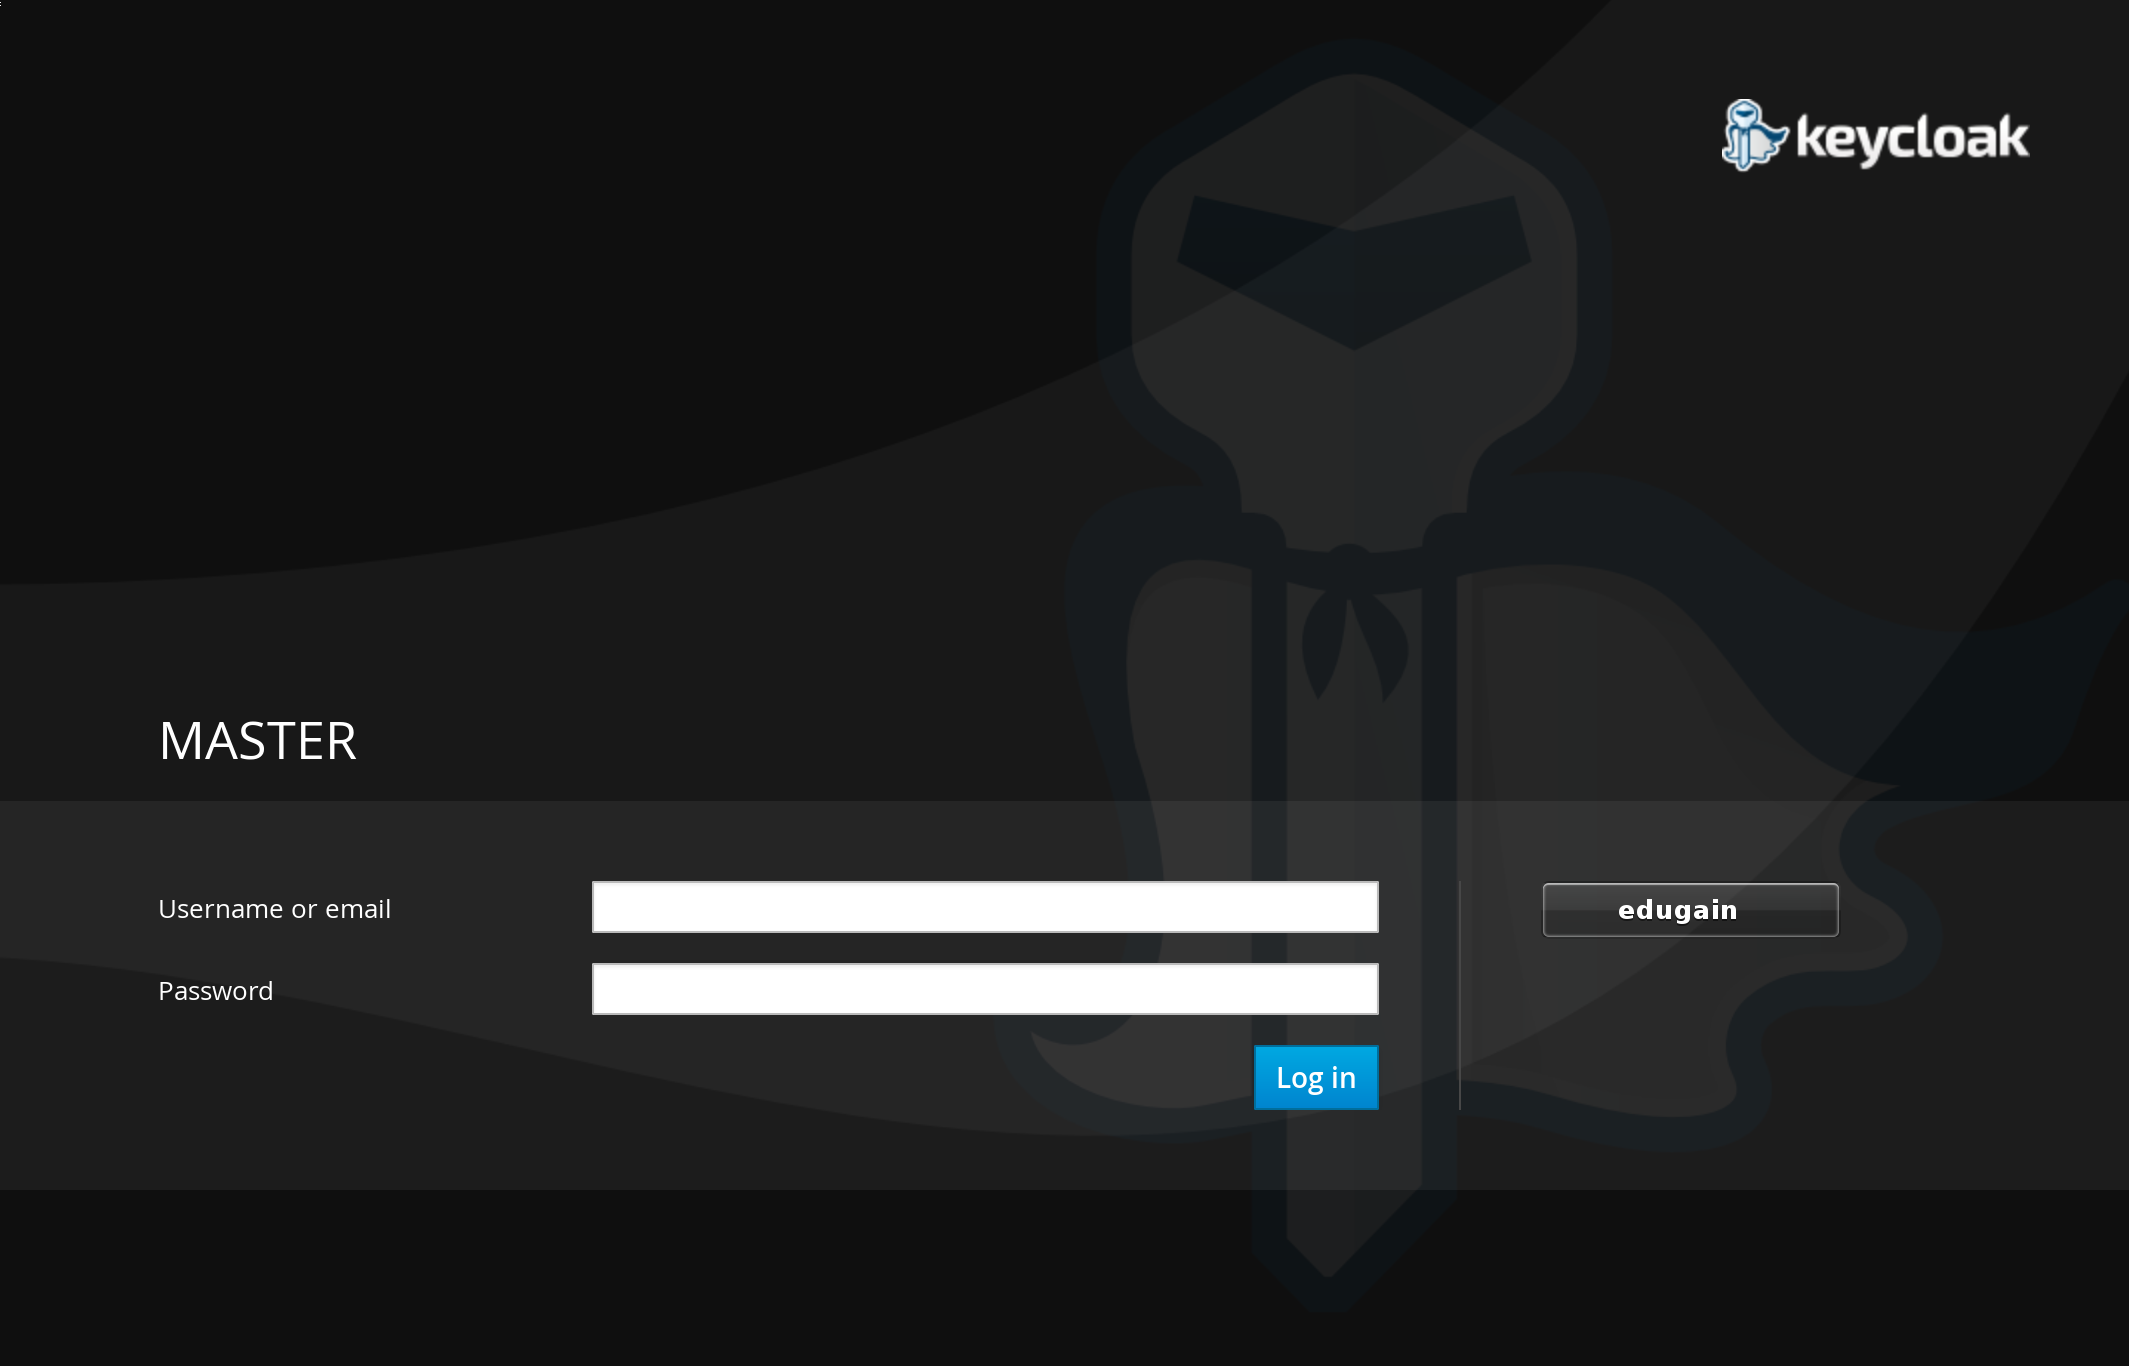
\includegraphics[width=\textwidth]{cyclone-federation-provider-login}\\
    Login screen to CYCLONE Federation Provider.
\end{center}


\vspace{0.5cm}

\section{Android}


\vspace{0.5cm}

\section{iOS}
